%%%%%%%%%%%%%%%%%%%%%%%%%%%%%%%%%%%%%%%%%%%%%%%%%%%%%%%%%%
\begin{frame}{The QoI Map Relates Inputs and Outputs}

\only<1>{

\begin{figure}[h]
	\includegraphics[width=0.85\textwidth]{./figures/threelevels/schematic_lambda_solution_data.pdf}
\end{figure}

}

\only<2>{

\begin{figure}[h]
	\includegraphics[width=0.85\textwidth]{./figures/threelevels/schematic_lambda_data.pdf}
\end{figure}

}

\only<3>{

\begin{figure}[h]
	\includegraphics[width=0.85\textwidth]{./figures/threelevels/schematic_lambda_data_level1.pdf}
\end{figure}

}

\end{frame}

%%%%%%%%%%%%%%%%%%%%%%%%%%%%%%%%%%%%%%%%%%%%%%%%%%%%%%%%%%
\begin{frame}{A Forward UQ Problem}

\begin{figure}[h]
	\includegraphics[width=0.85\textwidth]{./figures/threelevels/schematic_lambda_data_level3.pdf}
\end{figure}

{We denote the measurable spaces of parameters and data on the QoI as $(\pspace,\pborel)$ and $(\dspace,\dborel)$, respectively.}
\bigskip

\tdeepred{Given some prior density $\initial$ on $(\pspace,\pborel)$, we let $\predicted$ denote the push-forward of this density on $(\dspace,\dborel)$.}

\end{frame}

%%%%%%%%%%%%%%%%%%%%%%%%%%%%%%%%%%%%%%%%%%%%%%%%%%%%%%%%%%
\begin{frame}{The Inverse QoI Map}

\begin{figure}[h]
	\includegraphics[width=0.85\textwidth]{./figures/threelevels/schematic_data_lambda_level1.pdf}
\end{figure}

\end{frame}

%%%%%%%%%%%%%%%%%%%%%%%%%%%%%%%%%%%%%%%%%%%%%%%%%%%%%%%%%%
\begin{frame}{An Inverse UQ Problem}

\begin{figure}[h]
	\includegraphics[width=0.85\textwidth]{./figures/threelevels/schematic_data_lambda_level3.pdf}
\end{figure}

\tdeepred{Given $\obs$ on $(\dspace,\dborel)$, we let $\predicted$ denote the pullback (consistent) density on $(\pspace,\pborel)$.}

\end{frame}



\subsection{The Stochastic Inverse Problem}
%%%%%%%%%%%%%%%%%%%%%%%%%%%%%%%%%%%%%%%%%%%%%%%%%%%%%%%%%%
\begin{frame}[t]

\begin{figure}
\centering
	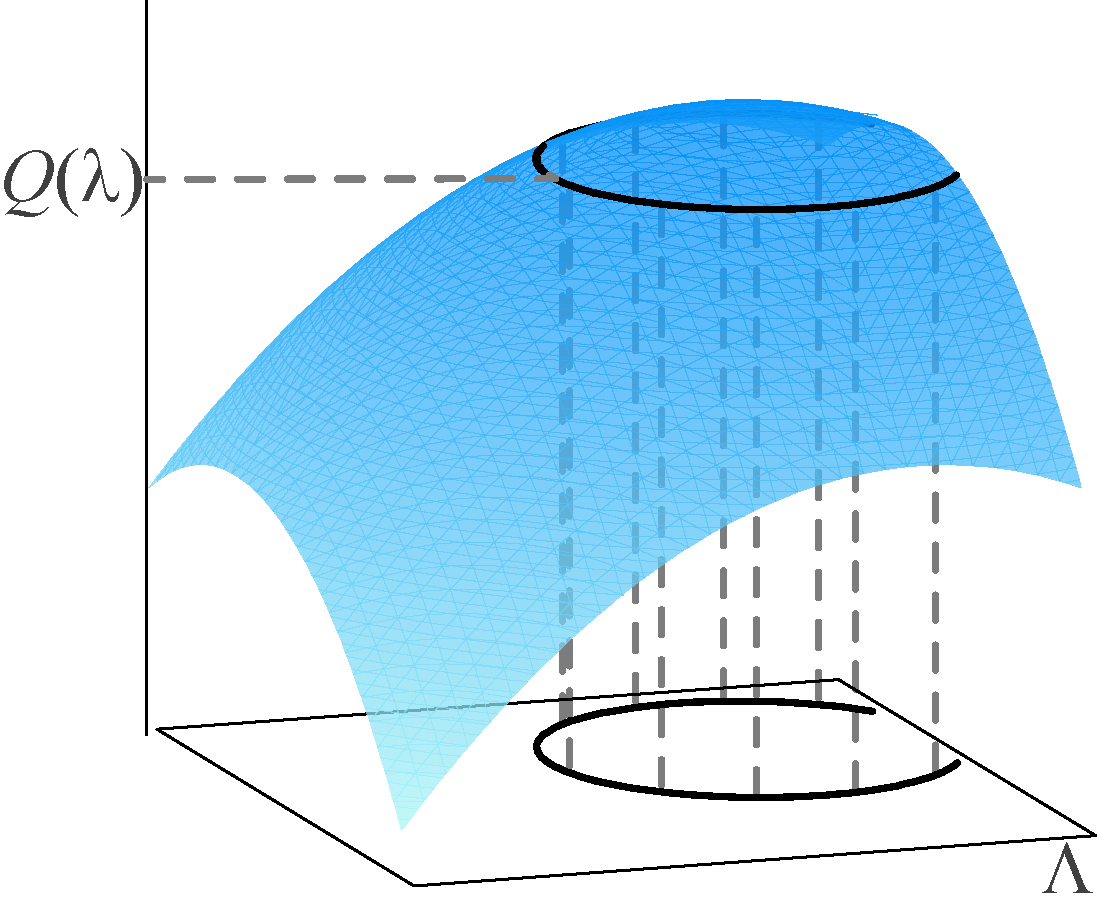
\includegraphics[width=.65\textwidth]{images/illustration1.pdf}<1>
	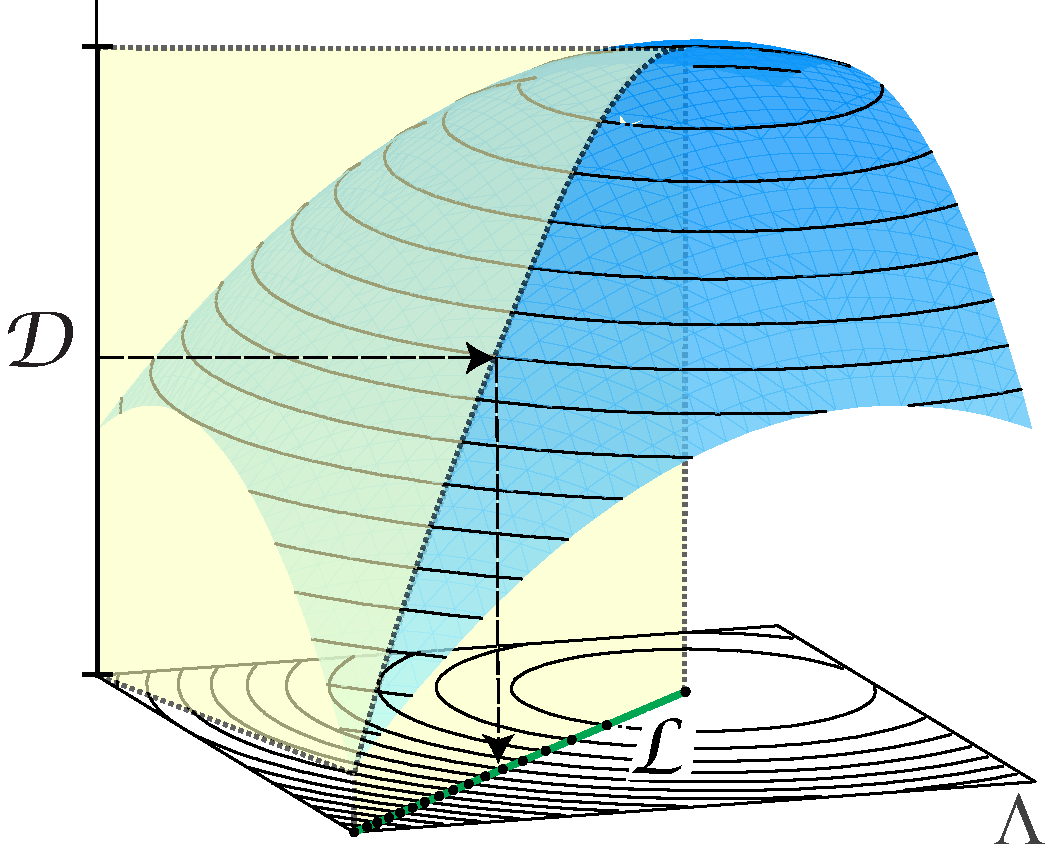
\includegraphics[width=.65\textwidth]{images/illustration2.pdf}<2>
	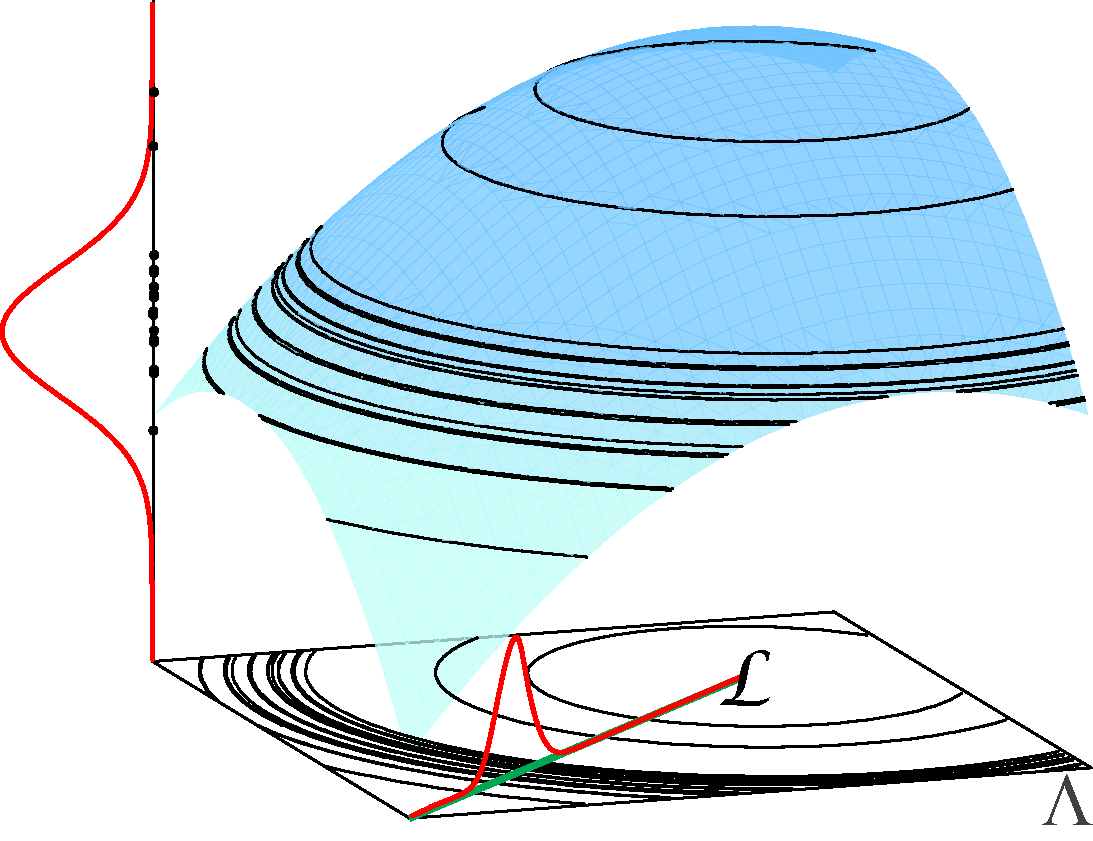
\includegraphics[width=.7\textwidth]{images/illustration3.pdf}<3>
\end{figure}
\begin{center}
{\scriptsize Figure adopted from \cite{BET14+} and used with permission}
\end{center}
\end{frame}

%%%%%%%%%%%%%%%%%%%%%%%%%%%%%%%%%%%%%%%%%%%%%%%%%%%%%%%%%%
\begin{frame}[t]

\begin{figure}
\centering
	\includegraphics[width=1\textwidth]{images/troy_mt3contour.png}
\end{figure}
\begin{center}

{\scriptsize Figure adopted from \cite{BET14+} and used with permission}

\tdeepred{Key Question:} Distinguish (assign probability to) events that belong to same contour.
\end{center}
\end{frame}
